%% abtex2-modelo-artigo.tex, v-1.9.5 laurocesar
%% Copyright 2012-2015 by abnTeX2 group at http://www.abntex.net.br/ 
%%
%% This work may be distributed and/or modified under the
%% conditions of the LaTeX Project Public License, either version 1.3
%% of this license or (at your option) any later version.
%% The latest version of this license is in
%%   http://www.latex-project.org/lppl.txt
%% and version 1.3 or later is part of all distributions of LaTeX
%% version 2005/12/01 or later.
%%
%% This work has the LPPL maintenance status `maintained'.
%% 
%% The Current Maintainer of this work is the abnTeX2 team, led
%% by Lauro César Araujo. Further information are available on 
%% http://www.abntex.net.br/
%%
%% This work consists of the files abntex2-modelo-artigo.tex and
%% abntex2-modelo-references.bib
%%

% ------------------------------------------------------------------------
% ------------------------------------------------------------------------
% abnTeX2: Modelo de Artigo Acadêmico em conformidade com
% ABNT NBR 6022:2003: Informação e documentação - Artigo em publicação 
% periódica científica impressa - Apresentação
% ------------------------------------------------------------------------
% ------------------------------------------------------------------------

\documentclass[
	% -- opções da classe memoir --
	article,			% indica que é um artigo acadêmico
	11pt,				% tamanho da fonte
	oneside,			% para impressão apenas no verso. Oposto a twoside
	a4paper,			% tamanho do papel. 
	% -- opções da classe abntex2 --
	%chapter=TITLE,		% títulos de capítulos convertidos em letras maiúsculas
	%section=TITLE,		% títulos de seções convertidos em letras maiúsculas
	%subsection=TITLE,	% títulos de subseções convertidos em letras maiúsculas
	%subsubsection=TITLE % títulos de subsubseções convertidos em letras maiúsculas
	% -- opções do pacote babel --
	english,			% idioma adicional para hifenização
	brazil,				% o último idioma é o principal do documento
	sumario=tradicional
	]{abntex2-inep-ufsc-bancada}


% ---
% PACOTES
% ---

% ---
% Pacotes fundamentais 
% ---
\usepackage{lmodern}			% Usa a fonte Latin Modern
\usepackage[T1]{fontenc}		% Selecao de codigos de fonte.
\usepackage[utf8]{inputenc}		% Codificacao do documento (conversão automática dos acentos)
\usepackage{indentfirst}		% Indenta o primeiro parágrafo de cada seção.
\usepackage{nomencl} 			% Lista de simbolos
\usepackage{color}				% Controle das cores
\usepackage{graphicx}			% Inclusão de gráficos
\usepackage{microtype} 			% para melhorias de justificação
\usepackage{datetime}           % Tempo e hora.
\usepackage{epstopdf}
% ---
		
% ---
% Pacotes adicionais, usados apenas no âmbito do Modelo Canônico do abnteX2
% ---
\usepackage{lipsum}				% para geração de dummy text
% ---
		
% ---
% Pacotes de citações
% ---
\usepackage[brazilian,hyperpageref]{backref}	 % Paginas com as citações na bibl
\usepackage[alf]{abntex2cite}	% Citações padrão ABNT
% ---

\usepackage{listings}
\usepackage{amsmath}		
\usepackage{amssymb}
\usepackage{mathrsfs}
\usepackage{booktabs} % Para Tabelas
\usepackage{subfig}  % permite ter subfiguras
\usepackage{float}
\usepackage{tikz,pgfplots}
\usepackage{pdfpages}
\usepackage{longtable}

\definecolor{dkgreen}{rgb}{0,0.6,0}
\definecolor{gray}{rgb}{0.5,0.5,0.5}
\definecolor{mauve}{rgb}{0.58,0,0.82}

\lstset{frame=tb,
	language=Matlab,
	aboveskip=3mm,
	belowskip=3mm,
	showstringspaces=false,
	columns=flexible,
	basicstyle={\small\ttfamily},
	numbers=none,
	numberstyle=\tiny\color{gray},
	keywordstyle=\color{blue},
	keepspaces=true,
	commentstyle=\color{dkgreen},
	stringstyle=\color{mauve},
	breaklines=true,
	breakatwhitespace=true,
	tabsize=3,
	texcl=true
}

% ---
% Configurações do pacote backref
% Usado sem a opção hyperpageref de backref
\renewcommand{\backrefpagesname}{Citado na(s) página(s):~}
% Texto padrão antes do número das páginas
\renewcommand{\backref}{}
% Define os textos da citação
\renewcommand*{\backrefalt}[4]{
	\ifcase #1 %
	Nenhuma citação no texto.%
	\or
	Citado na página #2.%
	\else
	Citado #1 vezes nas páginas #2.%
	\fi}%
% ---


% ---
% Informações de dados para CAPA e FOLHA DE ROSTO
% ---
\titulo{Modelo Canônico de relatório de bancada com \abnTeX}
\autor{Nome do Autor}
\local{Brasil}
\data{\today}
\universidade{UNIVERSIDADE FEDERAL DE SANTA CATARINA}
\programa{Pós--graduação em Engenharia Elétrica}
\laboratorio{INEP -- Instituto de Eletrônica de Potência}
\tipotrabalho{Relatório de Experimento}

\matricula{20150713}
\orientador{ Nome do Orientador}
\coorientador{ Nome do Coorientador}
\codexp{Exp03} % Código do experimento

% ---


% ---
% Configurações de aparência do PDF final

% alterando o aspecto da cor azul
\definecolor{blue}{RGB}{41,5,195}

% informações do PDF
\makeatletter
\hypersetup{
     	%pagebackref=true,
		pdftitle={\@title}, 
		pdfauthor={\@author},
    	pdfsubject={Modelo de artigo científico com abnTeX2},
	    pdfcreator={LaTeX with abnTeX2},
		pdfkeywords={abnt}{latex}{abntex}{abntex2}{atigo científico}, 
		colorlinks=true,       		% false: boxed links; true: colored links
    	linkcolor=blue,          	% color of internal links
    	citecolor=blue,        		% color of links to bibliography
    	filecolor=magenta,      		% color of file links
		urlcolor=blue,
		bookmarksdepth=4
}
\makeatother
% --- 

% ---
% compila o indice
% ---
\makeindex
% ---

% ---
% Altera as margens padrões
% ---
\setlrmarginsandblock{3cm}{3cm}{*}
\setulmarginsandblock{3cm}{3cm}{*}
\checkandfixthelayout
% ---

%%criar um novo estilo de cabeçalhos e rodapés
\makepagestyle{meuestilo}

%%cabeçalhos
\makeevenhead{meuestilo}
{Experimento X} %%pagina par
{}
{Página \thepage\ de \thelastpage}
\makeoddhead{meuestilo} %%pagina ímpar ou com oneside
{\imprimirtipotrabalho }
{}
{Página \thepage\ de \thelastpage}
\makeheadrule{meuestilo}{\textwidth}{\normalrulethickness} %linha
\makefootrule{meuestilo}{\textwidth}{\normalrulethickness}{1pt}

%% rodapé
\makeevenfoot{meuestilo} %%pagina par
{\today}
{}
{\currenttime h}
\makeoddfoot{meuestilo} %%pagina ímpar ou com oneside
{\today}
{}
{\currenttime h}


% --- 
% Espaçamentos entre linhas e parágrafos 
% --- 

% O tamanho do parágrafo é dado por:
\setlength{\parindent}{1.3cm}

% Controle do espaçamento entre um parágrafo e outro:
\setlength{\parskip}{0.2cm}  % tente também \onelineskip

% Espaçamento simples
\SingleSpacing

% ----
% Início do documento
% ----
\begin{document}

% Seleciona o idioma do documento (conforme pacotes do babel)
%\selectlanguage{english}
\selectlanguage{brazil}

% Retira espaço extra obsoleto entre as frases.
\frenchspacing 

%\pagestyle{meuestilo}
 
% ----------------------------------------------------------
% ELEMENTOS PRÉ-TEXTUAIS
% ----------------------------------------------------------

%---
%
% Se desejar escrever o artigo em duas colunas, descomente a linha abaixo
% e a linha com o texto ``FIM DE ARTIGO EM DUAS COLUNAS''.
% \twocolumn[    		% INICIO DE ARTIGO EM DUAS COLUNAS
%
%---
% página de titulo

\imprimircabecalho




% ]  				% FIM DE ARTIGO EM DUAS COLUNAS
% ---

% ----------------------------------------------------------
% ELEMENTOS TEXTUAIS
% ----------------------------------------------------------
\textual
\pagestyle{meuestilo}

% ----------------------------------------------------------
% Introdução
% ----------------------------------------------------------
\section*{Introdução}
\addcontentsline{toc}{section}{Introdução}

Este documento e seu código-fonte são exemplos de referência de uso da classe
\textsf{abntex2} e do pacote \textsf{abntex2cite}. O documento exemplifica a
elaboração de publicação periódica científica impressa produzida conforme a ABNT
NBR 6022:2003 \emph{Informação e documentação - Artigo em publicação periódica
científica impressa - Apresentação}.

A expressão ``Modelo canônico'' é utilizada para indicar que \abnTeX\ não é
modelo específico de nenhuma universidade ou instituição, mas que implementa tão
somente os requisitos das normas da ABNT. Uma lista completa das normas
observadas pelo \abnTeX\ é apresentada em \citeonline{abntex2classe}.

Sinta-se convidado a participar do projeto \abnTeX! Acesse o site do projeto em
\url{http://www.abntex.net.br/}. Também fique livre para conhecer,
estudar, alterar e redistribuir o trabalho do \abnTeX, desde que os arquivos
modificados tenham seus nomes alterados e que os créditos sejam dados aos
autores originais, nos termos da ``The \LaTeX\ Project Public
License''\footnote{\url{http://www.latex-project.org/lppl.txt}}.

Encorajamos que sejam realizadas customizações específicas deste documento.
Porém, recomendamos que ao invés de se alterar diretamente os arquivos do
\abnTeX, distribua-se arquivos com as respectivas customizações. Isso permite
que futuras versões do \abnTeX~não se tornem automaticamente incompatíveis com
as customizações promovidas. Consulte \citeonline{abntex2-wiki-como-customizar}
par mais informações.

Este exemplo deve ser utilizado como complemento do manual da classe
\textsf{abntex2} \cite{abntex2classe}, dos manuais do pacote
\textsf{abntex2cite} \cite{abntex2cite,abntex2cite-alf} e do manual da classe
\textsf{memoir} \cite{memoir}. Consulte o \citeonline{abntex2modelo} para obter
exemplos e informações adicionais de uso de \abnTeX\ e de \LaTeX.

% ----------------------------------------------------------
% Seção de explicações
% ----------------------------------------------------------
\newpage
\section{Exemplos de comandos}


\subsection{Inserindo código fonte}

\begin{lstlisting}[caption={Leitura dos dados simulados e conversão para estados topológicos.},label={lst:leituradadossim}]
% Pré definições iniciais
nsub=3;  % Numero de Sunmódulos
nbits=2*nsub; % Numero de bits necessários para representar os estados
nlevels=2*nsub+1; % Numero total de níveis

% Leitura dos pontos gerados por simulação
time=data(1,:)'; % extrai vetor de tempo
PWM=logical(data(2:end,:))'; % Conversão dos pulsos PWM para estados lógicos

% Cria vetor de string binário com os estados correspondentes
binstates=num2str([PWM(:,1) PWM(:,3) PWM(:,5) PWM(:,7) PWM(:,9) PWM(:,11)]);
state=fi(bin2dec(binstates),0,nbits,0); % Objeto numérico de ponto-fixo
\end{lstlisting}

\subsection{Figuras}



\begin{figure}[!h]
	\centering
	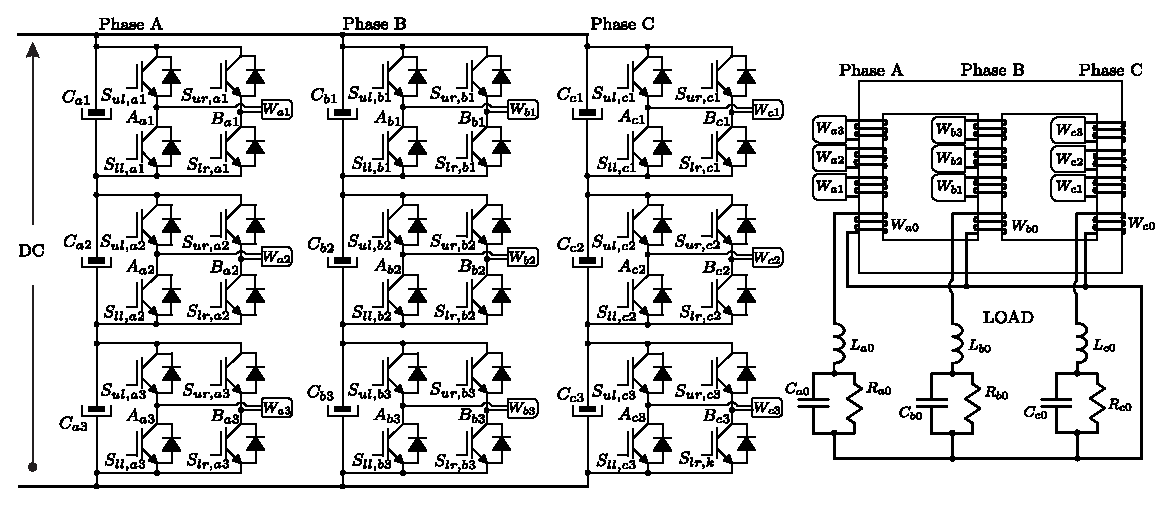
\includegraphics[width=1\linewidth]{figs/InversorTransformador}
	\caption{Conexão utilizada ao se empregar um transformador.}
	\label{fig:InversorTransformador}
\end{figure}


\subsection{Apresentando aquisições}


\begin{figure}[!h]
	\centering
	\begin{minipage}[t]{0.45\textwidth}	\centering
		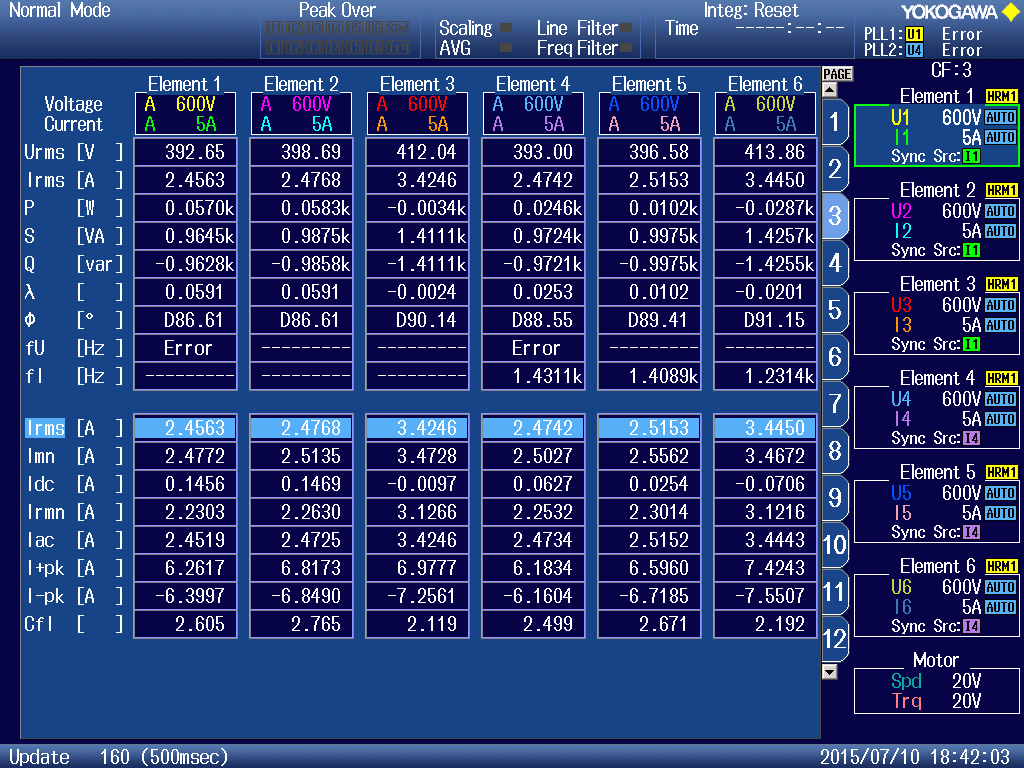
\includegraphics[width=1\linewidth]{aqs/0002}
		\caption{Tensões nos capacitores de barramento e correntes de saída dos inversores da fase B ($W_{b1}$, $W_{b2}$ e $W_{b3}$) e da fase A ($W_{a1}$, $W_{a2}$ e $W_{a3}$).}
		\label{fig:0002}
	\end{minipage}
	\quad
	\begin{minipage}[t]{0.45\textwidth} \centering
		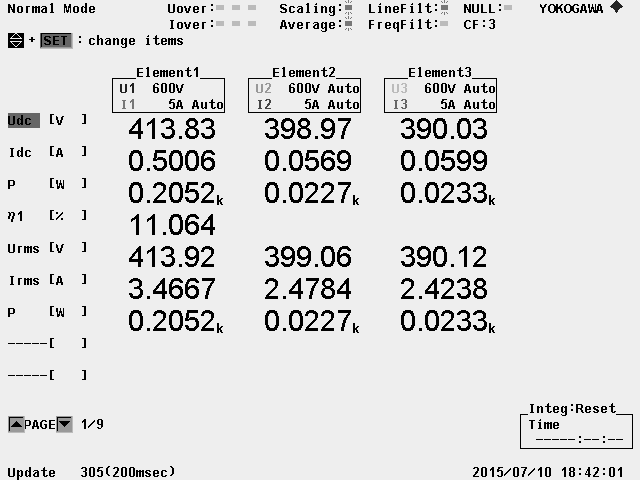
\includegraphics[width=1\linewidth]{aqs/TTZVSPWM0015}
		\caption{Tensões nos capacitores de barramento e correntes de saída dos inversores da fase C ($W_{c1}$, $W_{c2}$ e $W_{c3}$).}
		\label{fig:TTZVSPWM0015}
	\end{minipage}	
\end{figure}


\begin{figure}[!h]
	\centering
	\begin{minipage}[t]{0.45\textwidth}	\centering
		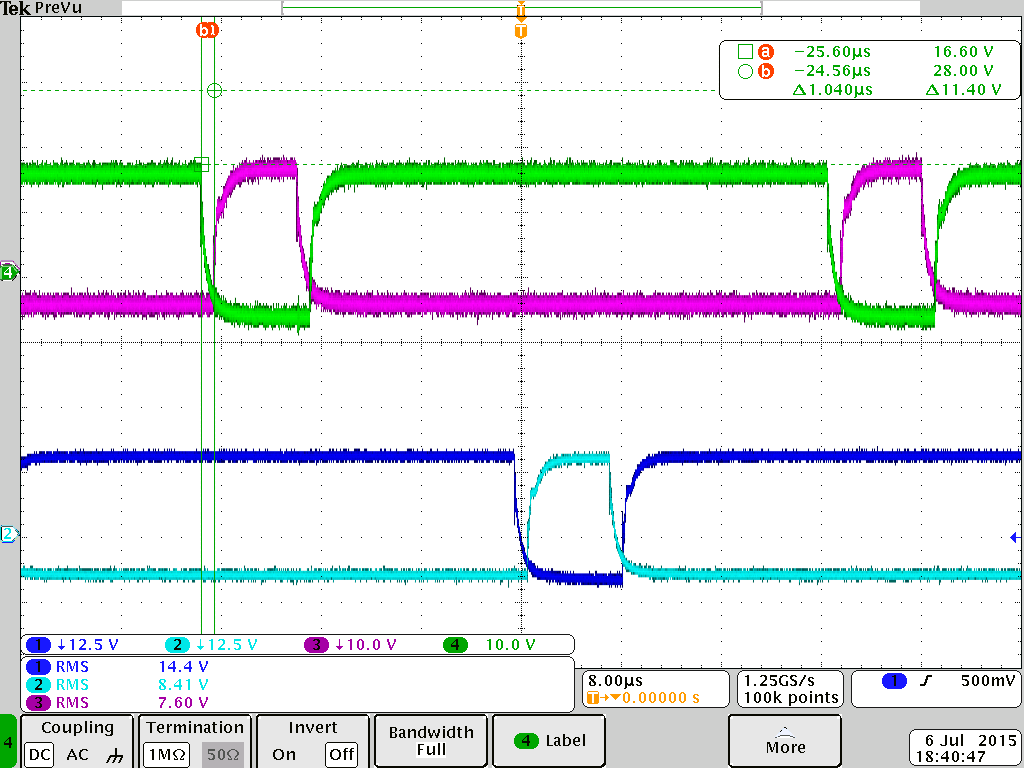
\includegraphics[width=1\linewidth]{aqs/tek0003}
		\caption{Tempo morto medido no braço 1 do inversor A3}
		\label{fig:tek0003}
	\end{minipage}
	\quad
	\begin{minipage}[t]{0.45\textwidth} 	\centering
		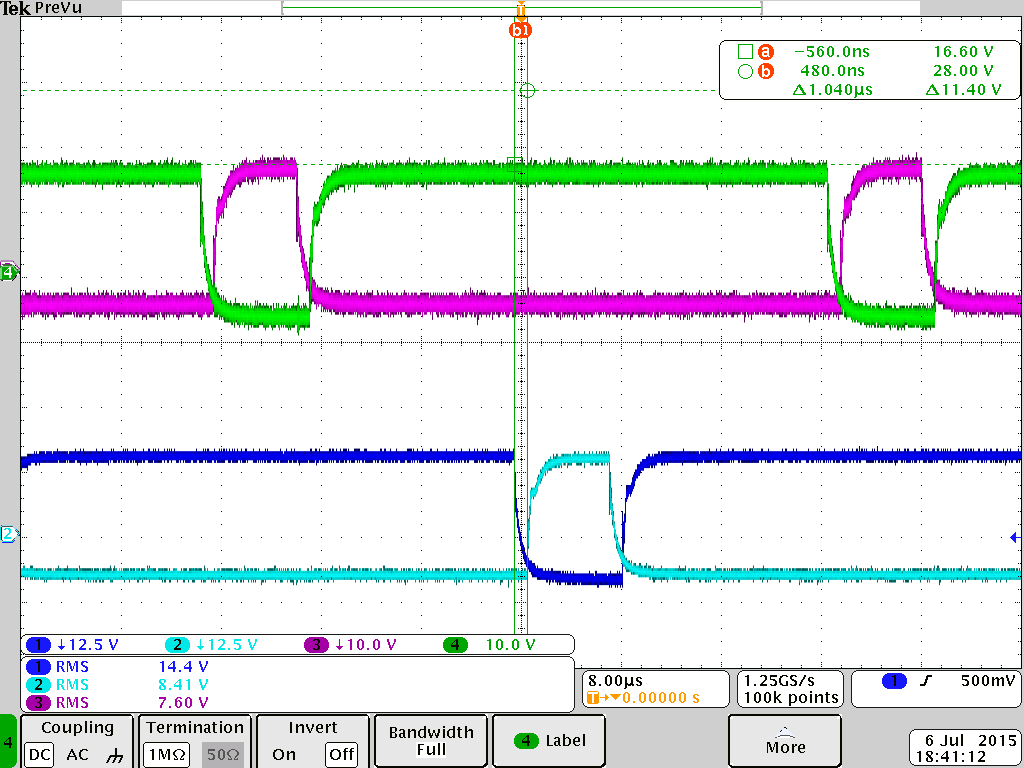
\includegraphics[width=1\linewidth]{aqs/tek0004}
		\caption{Tempo morto medido no braço 2 do inversor A3}
		\label{fig:tek0004}
	\end{minipage}	
\end{figure}


\begin{figure}[!h]
	\centering
	\begin{minipage}[t]{0.45\textwidth}	\centering
		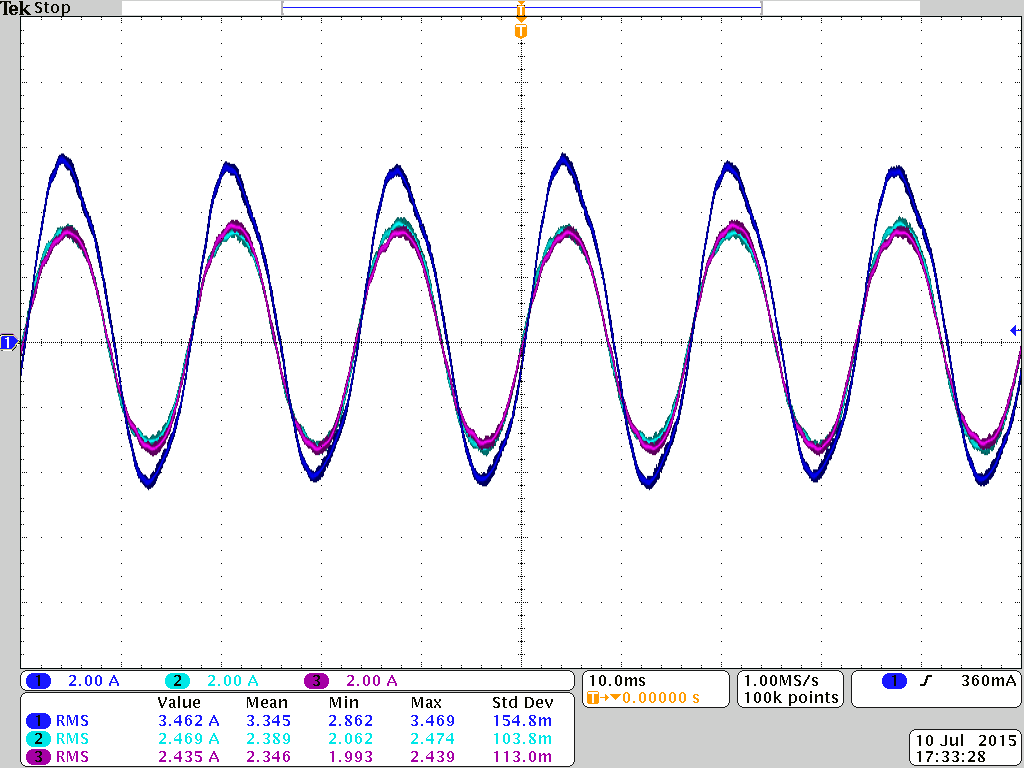
\includegraphics[width=1\linewidth]{aqs/tek0001}
		\caption{Correntes na fase C com um degrau de carga.}
		\label{fig:currenttek0001}
	\end{minipage}
	\quad
	\begin{minipage}[t]{0.45\textwidth} 	\centering
		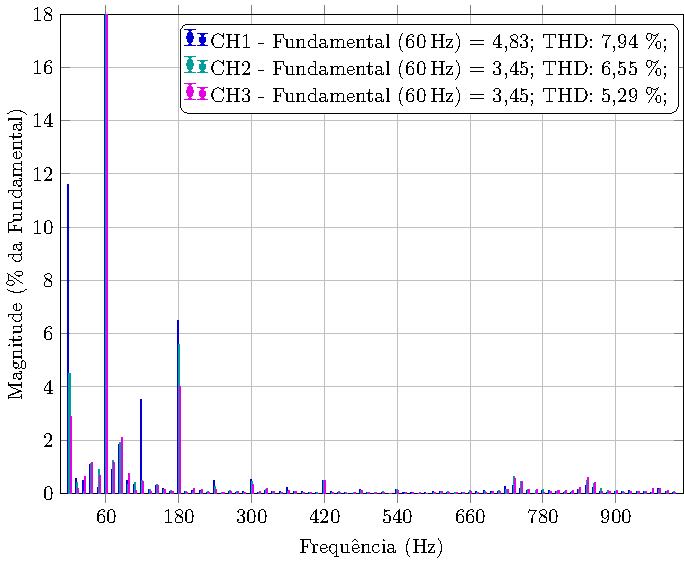
\includegraphics[width=1\linewidth]{aqs/tek0001FFT}
		\caption{Espectro das correntes na fase C com um degrau de carga.}
		\label{fig:currentFFTtek0001}
	\end{minipage}	
\end{figure}


\subsection{Margens}

A norma ABNT NBR 6022:2003 não estabelece uma margem específica a ser utilizada
no artigo científico. Dessa maneira, caso deseje alterar as margens, utilize os
comandos abaixo:

\begin{verbatim}
   \setlrmarginsandblock{3cm}{3cm}{*}
   \setulmarginsandblock{3cm}{3cm}{*}
   \checkandfixthelayout
\end{verbatim}

\subsection{Duas colunas}

É comum que artigos científicos sejam escritos em duas colunas. Para isso,
adicione a opção \texttt{twocolumn} à classe do documento, como no exemplo:

\begin{verbatim}
   \documentclass[article,11pt,oneside,a4paper,twocolumn]{abntex2}
\end{verbatim}

É possível indicar pontos do texto que se deseja manter em apenas uma coluna,
geralmente o título e os resumos. Os resumos em única coluna em documentos com
a opção \texttt{twocolumn} devem ser escritos no ambiente
\texttt{resumoumacoluna}:

\begin{verbatim}
   \twocolumn[              % INICIO DE ARTIGO EM DUAS COLUNAS

     \maketitle             % pagina de titulo

     \renewcommand{\resumoname}{Nome do resumo}
     \begin{resumoumacoluna}
        Texto do resumo.
      
        \vspace{\onelineskip}
 
        \noindent
        \textbf{Palavras-chave}: latex. abntex. editoração de texto.
     \end{resumoumacoluna}
   
   ]                        % FIM DE ARTIGO EM DUAS COLUNAS
\end{verbatim}

\subsection{Recuo do ambiente \texttt{citacao}}

Na produção de artigos (opção \texttt{article}), pode ser útil alterar o recuo
do ambiente \texttt{citacao}. Nesse caso, utilize o comando:

\begin{verbatim}
   \setlength{\ABNTEXcitacaorecuo}{1.8cm}
\end{verbatim}

Quando um documento é produzido com a opção \texttt{twocolumn}, a classe
\textsf{abntex2} automaticamente altera o recuo padrão de 4 cm, definido pela
ABNT NBR 10520:2002 seção 5.3, para 1.8 cm.

\section{Cabeçalhos e rodapés customizados}

Diferentes estilos de cabeçalhos e rodapés podem ser criados usando os
recursos padrões do \textsf{memoir}.

Um estilo próprio de cabeçalhos e rodapés pode ser diferente para páginas pares
e ímpares. Observe que a diferenciação entre páginas pares e ímpares só é
utilizada se a opção \texttt{twoside} da classe \textsf{abntex2} for utilizado.
Caso contrário, apenas o cabeçalho padrão da página par (\emph{even}) é usado.

Veja o exemplo abaixo cria um estilo chamado \texttt{meuestilo}. O código deve
ser inserido no preâmbulo do documento.

\begin{verbatim}
%%criar um novo estilo de cabeçalhos e rodapés
\makepagestyle{meuestilo}
  %%cabeçalhos
  \makeevenhead{meuestilo} %%pagina par
     {topo par à esquerda}
     {centro \thepage}
     {direita}
  \makeoddhead{meuestilo} %%pagina ímpar ou com oneside
     {topo ímpar/oneside à esquerda}
     {centro\thepage}
     {direita}
  \makeheadrule{meuestilo}{\textwidth}{\normalrulethickness} %linha
  %% rodapé
  \makeevenfoot{meuestilo}
     {rodapé par à esquerda} %%pagina par
     {centro \thepage}
     {direita} 
  \makeoddfoot{meuestilo} %%pagina ímpar ou com oneside
     {rodapé ímpar/onside à esquerda}
     {centro \thepage}
     {direita}
\end{verbatim}

Para usar o estilo criado, use o comando abaixo imediatamente após um dos
comandos de divisão do documento. Por exemplo:

\begin{verbatim}
   \begin{document}
     %%usar o estilo criado na primeira página do artigo:
     \pretextual
     \pagestyle{meuestilo}
     
     \maketitle
     ...
     
     %%usar o estilo criado nas páginas textuais
     \textual
     \pagestyle{meuestilo}
     
     \chapter{Novo capítulo}
     ...
   \end{document}  
\end{verbatim}
   
Outras informações sobre cabeçalhos e rodapés estão disponíveis na seção 7.3 do
manual do \textsf{memoir} \cite{memoir}.

\section{Mais exemplos no Modelo Canônico de Trabalhos Acadêmicos}

Este modelo de artigo é limitado em número de exemplos de comandos, pois são
apresentados exclusivamente comandos diretamente relacionados com a produção de
artigos.

Para exemplos adicionais de \abnTeX\ e \LaTeX, como inclusão de figuras,
fórmulas matemáticas, citações, e outros, consulte o documento
\citeonline{abntex2modelo}.

\section{Consulte o manual da classe \textsf{abntex2}}

Consulte o manual da classe \textsf{abntex2} \cite{abntex2classe} para uma
referência completa das macros e ambientes disponíveis.

% ---
% Finaliza a parte no bookmark do PDF, para que se inicie o bookmark na raiz
% ---
\bookmarksetup{startatroot}% 
% ---

% ---
% Conclusão
% ---
\section*{Considerações finais}
\addcontentsline{toc}{section}{Considerações finais}

\lipsum[1]

\begin{citacao}
\lipsum[2]
\end{citacao}

\lipsum[3]

% ----------------------------------------------------------
% ELEMENTOS PÓS-TEXTUAIS
% ----------------------------------------------------------
\postextual
\pagestyle{plain}

% ---
% Título e resumo em língua estrangeira
% ---

% \twocolumn[    		% INICIO DE ARTIGO EM DUAS COLUNAS



% ]  				% FIM DE ARTIGO EM DUAS COLUNAS
% ---

\newpage
% ----------------------------------------------------------
% Referências bibliográficas
% ----------------------------------------------------------
\bibliography{abntex2-modelo-references}

% ----------------------------------------------------------
% Glossário
% ----------------------------------------------------------
%
% Há diversas soluções prontas para glossário em LaTeX. 
% Consulte o manual do abnTeX2 para obter sugestões.
%
%\glossary

% ----------------------------------------------------------
% Apêndices
% ----------------------------------------------------------

\newpage
% ---
% Inicia os apêndices
% ---
\begin{apendicesenv}

% ----------------------------------------------------------
\chapter{Nullam elementum urna vel imperdiet sodales elit ipsum pharetra ligula
ac pretium ante justo a nulla curabitur tristique arcu eu metus}
% ----------------------------------------------------------
\lipsum[55-57]

\end{apendicesenv}
% ---

\newpage
% ----------------------------------------------------------
% Anexos
% ----------------------------------------------------------
\cftinserthook{toc}{AAA}
% ---
% Inicia os anexos
% ---
%\anexos
\begin{anexosenv}

\chapter{Datasheet para o conjunto inversor monofásico SPCIM 450-60-20}

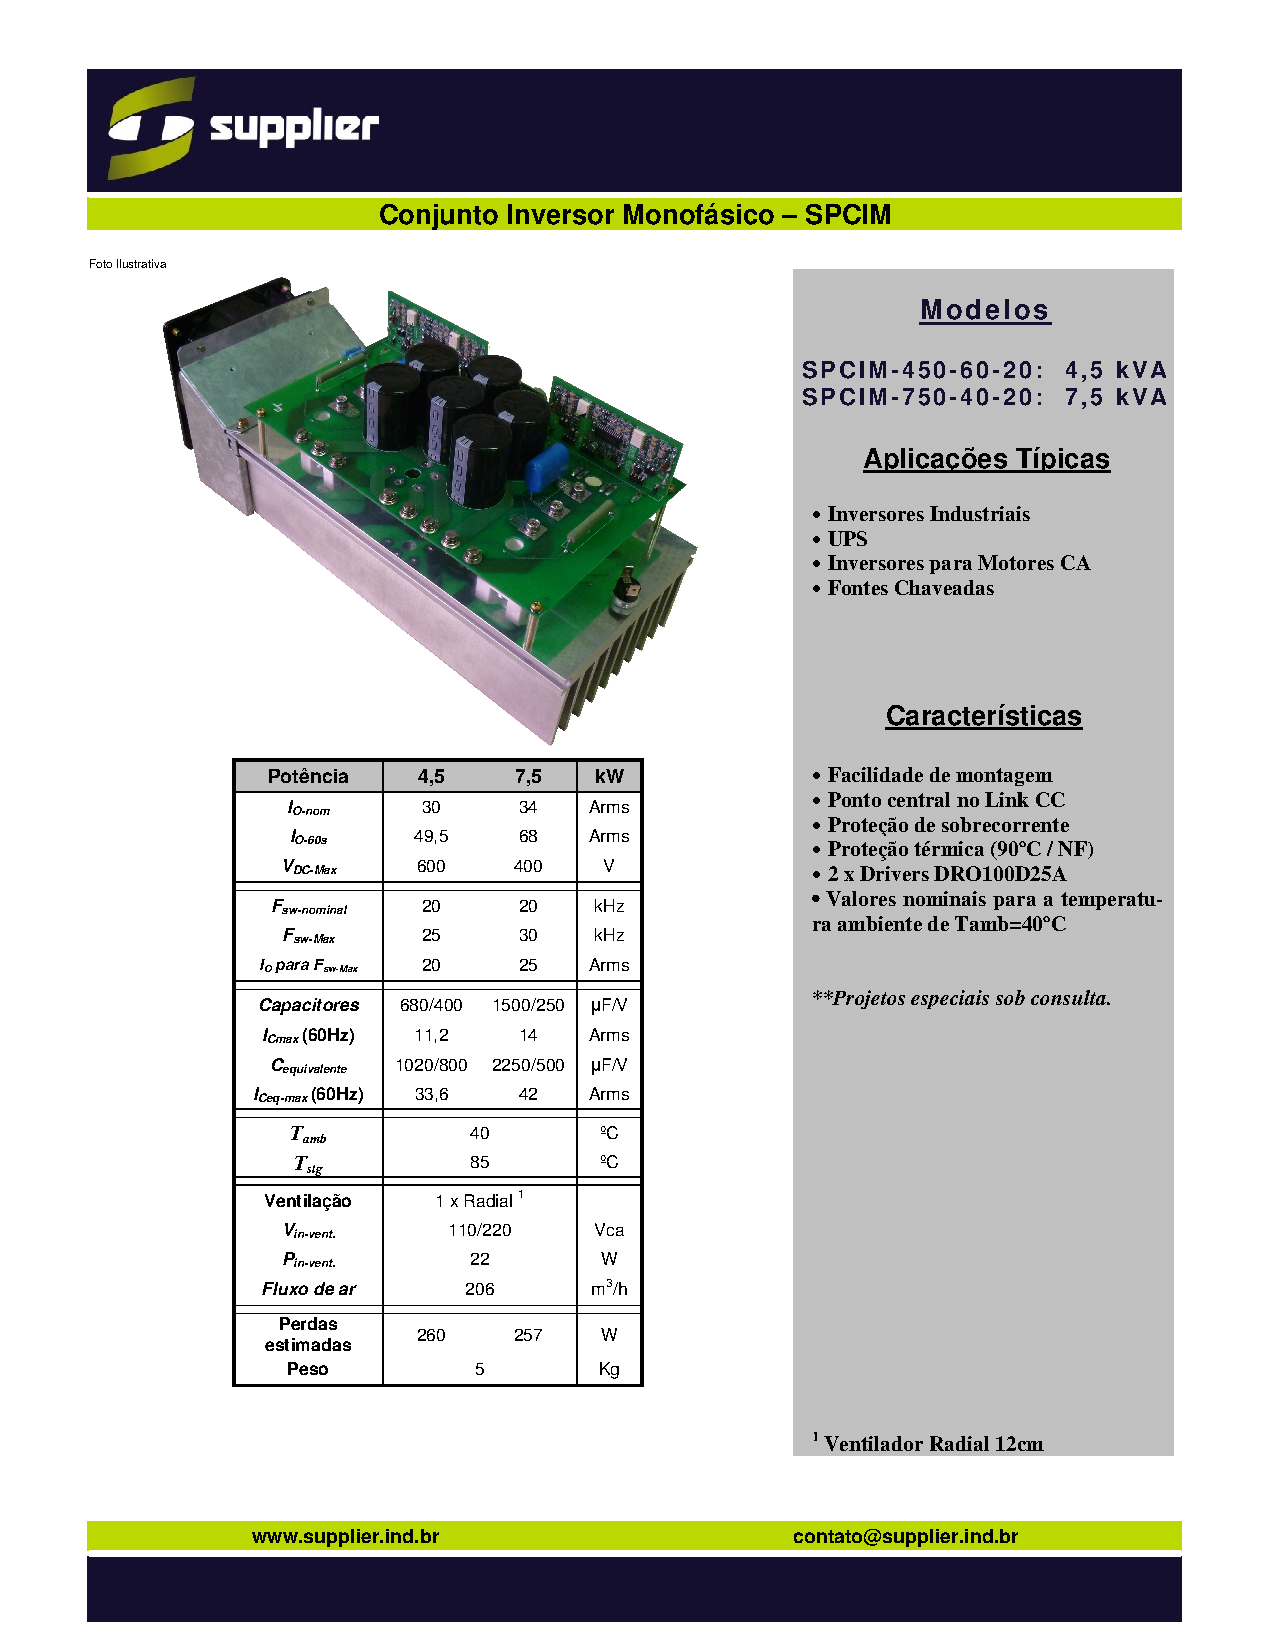
\includepdf[pages=-]{docs/SPCIM450-60-20.pdf}

\end{anexosenv}

\end{document}
